\documentclass[UTF8,a4paper,fontset=windows]{ctexart}
\usepackage{geometry}
\usepackage{multicol}
\usepackage{multirow}
\usepackage{tabu}
\usepackage{xeCJK}
\usepackage{CJK}
\usepackage{xeCJKfntef}
\usepackage{fancyhdr}
\usepackage{graphicx}
\usepackage{lastpage}
\usepackage{listings}
\usepackage{xcolor}
\usepackage{fontspec}
\usepackage{wrapfig}
\usepackage{layout}
\usepackage{graphicx}
\usepackage{float}
\usepackage{titletoc}
\usepackage[colorlinks,linkcolor=blue]{hyperref}

\newcommand\filename[1]{\emph{\textbf{#1}}}
\newcommand\udot[1]{\textbf{\color{black}\CJKunderdot{\color{black}#1}}}

\newcommand\newprob[3]{
    \newpage
    \pagestyle{fancy}
    \lhead{南宁市第三中学 2023 年科技节 \space \textit{程序设计竞赛} \space \texttt{NNSZCP-2023}} \rhead{\textbf{#1}  #2(#3)}
    \cfoot{第 \thepage 页 \qquad 共 \pageref{LastPage} 页}
    \phantomsection
    \addcontentsline{toc}{section}{#1  #2(#3)}
    \begin{center}
        \LARGE
        \textbf{#1  #2}(#3)
    \end{center}
    \large
}
\newcommand\para[1]{
    $ $ \\
    \textbf{【#1】}
    \phantomsection
    \addcontentsline{toc}{subsection}{【#1】}
}
\newcommand\sample[2]{
    $ $ \\
    \textbf{【样例} #1\textbf{#2】}
    \phantomsection
    \addcontentsline{toc}{subsection}{【样例 #1 #2】}
}
\setmonofont{Consolas}

\lstset{
    basicstyle={
        \color{black}
        \fontspec{Consolas}
    },
    keywordstyle={
        \color{blue}
        \fontspec{Consolas}
    },
    numberstyle={
        \color{gray}
        \fontspec{Consolas}
        \small
    },
    rulecolor=\color{blue},
    numbers=left,
    frame=single,
    morekeywords={Sample, Input, Output},
}


\geometry{left=2.52cm,right=2.52cm,top=2.5cm,bottom=2.5cm}
\begin{document}
    \pagestyle{fancy}
    \lhead{南宁市第三中学 2023 年科技节 程序设计竞赛} \rhead{}
    \cfoot{第 \thepage 页 \qquad 共 \pageref{LastPage} \color{black} 页}
    \thispagestyle{empty}
    \addcontentsline{toc}{section}{注意事项}
    \begin{center}
        \huge
        \textbf{南宁市第三中学 2023 年科技节}
        \\
        \LARGE
        \textit{程序设计竞赛}
        \\
        \texttt{NNSZCP-2023}
        \\
        \Large
        比赛时间:2023 年 11 月 26 日 00:00 $\sim$ 00:00
        \\
    \end{center}
    \large
    \begin{center}
        \begin{tabular}{cclccc}
			\hline
			\textbf{题目编号} & \textbf{题目中文名称} & \textbf{题目英文名称} & \textbf{时间限制} & \textbf{内存限制} & \textbf{子任务数量} \\ \hline
			\textbf{A} & 欢迎光临 & welcome & 1 秒 & 128 MiB & 3 \\
			\textbf{B} & 反应原理 & reaction & 1 秒 & 128 MiB & 3 \\
			\textbf{C} & 暮光闪闪 & twilight & 2 秒 & 256 MiB & 3 \\
			\textbf{D} & 中考录取 & exam & 1 秒 & 128 MiB & 2 \\
			\textbf{E} & 填数游戏 & game & 1 秒 & 128 MiB & 4 \\
			\textbf{F} & 初生几何 & mathematics & 2 秒 & 128 MiB & 2 \\
			\textbf{G} & 排序算法 & sort & 2 秒 & 256 MiB & 3 \\
			\textbf{H} & 购买车券 & sparkarte & 2 秒 & 256 MiB & 5 \\
			\textbf{I} & 花腔星云 & coloratura & 2 秒 & 256 MiB & 5 \\
			\textbf{J} & 妄想感伤 & sadness & 2 秒 & 512 MiB & 8 \\ \hline
		\end{tabular}
	\end{center}

\newprob{A}{欢迎光临}{welcome}

\para{题目背景}

南宁市第三中学是广西首批重点中学、广西首批示范性高中、首批普通高中新课程新教材实施国家级示范校。学校前身为 1897 年维新人士余镜清创办的南宁乌龙寺讲堂。学校目前拥有青山校区、五象校区、初中部青秀校区、初中部五象校区、初中部五象校区等 5 个校区,形成多校区集团办学模式。历经 126 年办学历史的洗礼与积淀,南宁三中以“真•爱教育”的办学思想和“德育为先,文理并重,崇尚一流”的办学特色饮誉华夏大地,成为莘莘学子向往的求知殿堂。

\para{题目描述}

为了欢迎各位新老选手的到来,南宁三中 01 社的成员们写了一句欢迎语。但是你作为一名新选手,不是很了解夹杂在欢迎语中的各种梗,你只知道 \texttt{nnsz} 是“南宁三中”的意思。

聪明的你想知道,在欢迎语中,是否存在一段连续部分(即子串)为 \texttt{nnsz}。

\para{输入格式}

给定一个字符串 $S$,代表欢迎语。

\para{输出格式}

如果欢迎语 $S$ 存在一段连续部分(即子串)为 \texttt{nnsz},输出 \texttt{yes},否则输出 \texttt{no}。

答案不区分大小写。

例如,当答案为 \texttt{yes} 时,\texttt{YES}、\texttt{yEs}、\texttt{YEs} 等答案均可被判定为正确答案。

\sample{1}{输入}

\begin{lstlisting}
welcometonnsz
\end{lstlisting}

\sample{1}{输出}

\begin{lstlisting}
yes
\end{lstlisting}

\sample{2}{输入}

\begin{lstlisting}
nnez
\end{lstlisting}

\sample{2}{输出}

\begin{lstlisting}
no
\end{lstlisting}

\sample{3}{输入}

\begin{lstlisting}
nocommander
\end{lstlisting}

\sample{3}{输出}

\begin{lstlisting}
no
\end{lstlisting}

\para{数据范围}

记 $ n $ 为 $ S $ 的长度。

对于 $ 100\% $ 的数据,保证 $ 1 \le n \le 100 $,且 $ S $ 中仅包含小写英文字母。

\begin{center}
	\begin{tabu}{c|c|c}
		\tabucline[2pt]{-}
		子任务编号 &  限制 & 分数 \\
		\tabucline[1.2pt]{-}
		Subtask 0 & $1 \le n \le 3$ & 45 \\ \hline
		Subtask 1 & $n = 4$ & 5  \\ \hline
		Subtask 2 & $1 \le n \le {10}^2$ & 50 \\
		\tabucline[2pt]{-}
	\end{tabu}
\end{center}

\newprob{B}{反应原理}{reaction}

\para{题目背景}

你说的对,但是《化学》是由化学家自主研发的一款全新开放世界冒险游戏。故事发生在一个被称作“微观状态”的架空世界,在这里,被选中的原子将被授予“电子”,导引键能之力。

你将扮演一位名为“臭写题的”的神秘角色,在自由的刷题中邂逅性质各异、能力独特的化合物们,和他们一起击败强题,找回失散的离子——同时,逐步发掘“元素周期表”的真相。

\para{题目描述}

小 P 的化学烂到了家。

我们知道:一个化学反应由多个反应步骤依次进行完成。

已知这个反应共有 $n$ 个反应步骤,初始时物质的总能量为 $a_0$,定义第 $i$ 个反应步骤后,物质的总能量为 $a_i$。

小 P 的化学老师告诉他:定义化学反应的\textit{活化能}是某个反应步骤进行前后,总能量\udot{变化量}的\udot{最大值},即 $\max_{i=0}^{n-1} \{a_{i + 1} - a_{i}\}$。

但是正如前文所言,小 P 记错了定义:定义化学反应的\textit{活化能}是整个化学反应进程中的能量的\udot{最大值},即 $\max_{i=0}^{n} \{a_i\}$。

请分别求出:在\udot{错误}定义和\udot{正确}定义下,这个反应的\textit{活化能}是多少?

\para{输入格式}

从标准输入读入数据。

第一行一个正整数 $n$,含义见题目描述。

接下来一行 $n + 1$ 个整数,第 $i$ 个整数代表 $a_{i - 1}$。

\para{输出格式}

输出到标准输出中。

两行分别包含一个整数,分别表示\udot{错误}定义和\udot{正确}定义下,反应的活化能。

\sample{1}{输入}

\begin{lstlisting}
4
1 4 6 10 12
\end{lstlisting}

\sample{1}{输出}

\begin{lstlisting}
12
4
\end{lstlisting}

\sample{1}{解释}

错误定义下的活化能为 $\max\{1, 4, 6, 10, 12\} = 12$。

正确定义下的活化能为 $\max\{4-1, 6-4, 10-6, 12-10\} = 4$。

\sample{2}{输入}

\begin{lstlisting}
4
31 12 23 13 -21
\end{lstlisting}

\sample{2}{输出}

\begin{lstlisting}
31
11
\end{lstlisting}

\para{数据范围}

对 $100\%$ 的数据,保证 $2 \le n \le 3 \times {10}^5$,$-{10}^7 \le a_i \le {10}^7$。

\begin{center}
	\begin{tabu}{c|c|c|c}
		\tabucline[2pt]{-}
		子任务编号 &  限制 & 特殊性质 & 分数 \\
		\tabucline[1.2pt]{-}
		Subtask 0 & $2 \le n \le {10}^3$ & 无 & 25 \\ \hline
		Subtask 1 & $2 \le n \le {10}^5$ & A & 25  \\ \hline
		Subtask 2 & $2 \le n \le 3 \times {10}^5$ & 无 & 50 \\
		\tabucline[2pt]{-}
	\end{tabu}
\end{center}

特殊性质 A:保证对 $0 \le i < n$,$a_i \le a_{i+1}$。

\newprob{C}{暮光闪闪}{twilight}

\para{题目背景}

\begin{figure}[H]
\centering

\includegraphics[scale=0.16]{./picture/twilight.jpg}
\end{figure}

\para{题目描述}

小马利亚要建造一批新的建筑,公主暮光闪闪一共计划了 $n$ 栋建筑物,每一栋建筑物的高度为 $h_i$。

现在,作为该工程的领导者,云宝希望城市的规划能够为天马们提供一些便利。具体地,一共 $m$ 匹天马中,对于第 $i$ 匹天马,其飞行的高度为 $s_i$。

对第 $i$ 匹天马,她想知道:这匹天马最多能够在多少对建筑之间穿梭?

由于工期紧张,她需要你的帮助,因此请你帮忙解决这个问题。

\para{输入格式}

第一行两个整数 $n,m$。

第二行 $n$ 个正整数,代表 $h_1,h_2,h_3, \cdots, h_n$。

第三行 $m$ 个正整数,代表 $s_1,s_2,s_3, \cdots, s_m$。

\para{输出格式}

一共 $m$ 行,每行一个整数,代表答案。

\sample{1}{输入}

\begin{lstlisting}
3 2
1 2 3
1 2
\end{lstlisting}

\sample{1}{输出}

\begin{lstlisting}
2
3
\end{lstlisting}

\sample{1}{解释}

对于 $ s_1 = 1 $ 的天马,它最多可以在以下 $ 2 $ 对建筑穿梭。

\begin{itemize}
\item 建筑 $ 1 $ 与建筑 $ 2 $;
\item 建筑 $ 2 $ 与建筑 $ 3 $。
\end{itemize}

对于 $ s_2 = 2 $ 的天马,它最多可以在以下 $ 3 $ 对建筑穿梭。

\begin{itemize}
\item 建筑 $ 1 $ 与建筑 $ 2 $;
\item 建筑 $ 1 $ 与建筑 $ 3 $;
\item 建筑 $ 2 $ 与建筑 $ 3 $。
\end{itemize}

\para{数据范围}

对于 $100\%$ 的数据,有 $1 \le n \le 2 \times 10^3$,$1 \le m \le 10^5$,$1 \le h_i, s_i \le 10^9$。

\begin{center}
	\begin{tabu}{c|c|c|c}
		\tabucline[2pt]{-}
		子任务编号 &  限制 & 特殊性质 & 分数 \\ \tabucline[1.2pt]{-}
		Subtask 0 & $1 \le n \le 100$,$1 \le m \le 100$ & 无 & 20 \\ \hline
		Subtask 1 & $1 \le n \le 2 \times 10^3$, $1 \le m \le 10^5$ & A & 10 \\ \hline
		Subtask 4 & $1 \le n \le 2 \times 10^3$,$1 \le m \le 10^5$ & 无 & 70 \\ \tabucline[2pt]{-}
	\end{tabu}
\end{center}

特殊性质 A:所有的 $h_i$ 均相等。

\newprob{D}{中考报名}{exam}

\para{题目描述}

N 市某年的初中学业考试和高中阶段学校招生考试成绩排名规则如下:

考生需经历语文、数学、英语、物理、化学、道德与法治和历史(以下简称“政史”)共 $ 6 $ 门文化课考试,以及体育考试。

考生在每门考试中都有对应的原始分(为简便起见,我们认为\udot{原始分都是整数}),我们设考生 $ i $ 的原始分为:

\begin{itemize}

\item 语文原始分为 $a_i$;
\item 数学原始分为 $b_i$;
\item 英语原始分为 $c_i$;
\item 物理原始分为 $d_i$;
\item 化学原始分为 $e_i$;
\item 政史原始分为 $f_i$;
\item 体育原始分为 $g_i$;
\item 总原始分为 $ s_i = a_i + b_i + c_i + d_i + e_i + f_i + g_i$。

\end{itemize}

对于语文原始分、数学原始分、英语原始分、物理原始分、化学原始分、政史原始分和总原始分共 $ 7 $ 项数据,每项数据都被\udot{从高到低}划分成 $ \texttt{A+} $,$ \texttt{A} $,$ \texttt{B+} $,$ \texttt{B} $,$ \texttt{C+} $,$ \texttt{C} $,$ \texttt{D} $,$ \texttt{E} $ 共 $ 8 $ 种等级,但为问题简便起见,我们认为\udot{等级只有 $ \texttt{A+} $ 与 $ \texttt{A} $ 共 $ 2 $ 种}。

对于每一项数据,教育部门划定了一条分数线 $ l $。以语文学科为例,设教育部门为语文学科划定的分数线为 $ l_a $,则对于考生 $ i $,有:

\begin{itemize}

\item 当 $ a_i < l_a $ 时,考生 $ i $ 的语文等级为 $ \texttt{A} $;
\item 当 $ a_i \ge l_a $ 时,考生 $ i $ 的语文等级为 $ \texttt{A+} $;
\item 其他科目的对应等级以同样方式评定。

\end{itemize}

在对每个考生的原始分划分等级后,两名考生的等级组合将按如下规则比较:

\begin{itemize}

\item 两名考生中\udot{总分等级}更高的一名的成绩更优;
\item 若两名考生的总分等级相同,则两名考生中 $ \texttt{A+} $ 等级的\udot{数量}更多的一名的成绩更优;
\item 若两名考生的 $ \texttt{A+} $ 等级的数量仍相同,则\udot{语文等级}更高的一名的成绩更优;
\item 若两名考生的语文等级仍相同,则\udot{数学等级}更高的一名的成绩更优;
\item 若两名考生的数学等级仍相同,则\udot{英语等级}更高的一名的成绩更优;
\item 若两名考生的英语等级仍相同,则\udot{物理等级}更高的一名的成绩更优;
\item 若两名考生的物理等级仍相同,则\udot{化学等级}更高的一名的成绩更优;
\item 若两名考生的化学等级仍相同,则\udot{政史等级}更高的一名的成绩更优;
\item 若两名考生的政史等级仍相同,则直接认为两名考生的成绩\udot{完全相同},没有优劣之分(\udot{尽管两人的原始分可能不完全相同})。

\end{itemize}

ZSNN 作为 N 市的一所重点高中,是众多优秀学子所向往的学府。自然,想要进入 ZSNN,就要经过激烈的竞争。

该年报考 ZSNN 的考生共有 $ n $ 名,而 ZSNN 拟录取的新生人数为 $ m $ 人。而教育部门规定,\udot{成绩组合完全相同的人,其报考结果(即录取与否)也应该相同}。这导致了实际录取人数 $ m^\prime $ 与拟录取人数 $ m $ 可能略有出入。

现在,给出 $ n $ 和 $ m $,以及 $ n $ 名考生的所有原始分数据,和各个科目的分数线。请你求出在保证 $ m^\prime \ge m $ 的情况下 $ m^\prime $ 的\udot{最小值}。

\udot{请注意:题目中的考试规则定义可能与实际生活略有出入,请以文中的规则为准。}

\para{输入格式}

从标准输入读入数据。

第一行包含 $ 7 $ 个整数 $ l_a, l_b, l_c, l_d, l_e, l_f, l_s $,分别代表语文、数学、英语、物理、化学、政史和总分的分数线。

第二行包含 $ 2 $ 个整数 $ n $ 和 $ m $,分别代表报考 ZSNN 的考生总数和 ZSNN 拟录取的新生人数。

接下来的 $ n $ 行中的第 $ i $ 行包含 $ 7 $ 个整数 $ a_i, b_i, c_i, d_i, e_i, f_i, g_i $,分别代表第 $ i $ 名考生的语文、数学、英语、物理、化学、政史、体育原始分。

\para{输出格式}

输出到标准输出中。

输出一个整数 $ m^\prime $,代表实际录取的新生人数。

\sample{1}{输入}

\begin{lstlisting}
105 106 117 93 97 118 640
2 1
110 113 119 95 98 119 60
105 106 117 93 97 118 36
\end{lstlisting}

\sample{1}{输出}

\begin{lstlisting}
2
\end{lstlisting}

\sample{1}{解释}

考生 $ 1 $ 与考生 $ 2 $ 的等级组合均为“总分 $ \texttt{A+} $ 和 $ \texttt{6A+} $”,他们应该同时被录取。

\sample{2}{输入}

\begin{lstlisting}
105 106 117 93 97 118 640
2 1
100 106 115 92 95 114 57
104 105 116 93 96 117 60
\end{lstlisting}

\sample{2}{输出}

\begin{lstlisting}
1
\end{lstlisting}

\sample{2}{解释}

考生 $ 1 $ 与考生 $ 2 $ 的等级组合均为“总分 $ \texttt{A+} $ 和 $ \texttt{1A+5A} $”,但在两人语文等级相同的情况下,考生 $ 1 $ 的数学等级高于 $ 2 $ 考生 $ 2 $ 的数学等级。故考生 $ 1 $ 的成绩更优秀,只有考生 $ 1 $ 能被录取。

\sample{3}{输入}

\begin{lstlisting}
105 106 117 93 97 118 640
2 1
104 105 116 92 96 117 60
120 120 120 100 100 0 60
\end{lstlisting}

\sample{3}{输出}

\begin{lstlisting}
1
\end{lstlisting}

\sample{3}{解释}

考生 $ 1 $ 的总分等级为 $ \texttt{A+} $,而考生 $ 2 $ 的总分等级为 $ \texttt{A} $。故考生 $ 1 $ 的成绩更优秀,只有考生 $ 1 $ 能被录取。

\sample{4}{输入}

\begin{lstlisting}
81 55 33 22 84 5 180
10 3
26 45 51 65 60 1 2
105 69 18 40 24 40 4
54 44 9 85 10 114 11
41 62 69 82 98 52 53
109 78 88 24 91 60 13
103 99 11 73 53 66 0
69 104 63 45 38 92 17
43 119 75 94 6 119 33
76 101 50 12 8 70 51
54 48 21 79 73 27 25
\end{lstlisting}

\sample{4}{输出}

\begin{lstlisting}
4
\end{lstlisting}

\para{数据范围}

对于 $ 100\% $ 的数据,保证 $ 1 \le m \le n \le 10^5 $,$ 0 \le a_i, l_a \le 120 $,$ 0 \le b_i, l_b \le 120 $,$ 0 \le c_i, l_c \le 120 $,$ 0 \le d_i, l_d \le 100 $,$ 0 \le e_i, l_e \le 100 $,$ 0 \le f_i, l_f \le 120 $,$ 0 \le g_i \le 60 $,$ 0 \le l_s \le 740 $,且所有输入数据均为整数。

\begin{center}
	\begin{tabu}{c|c|c|c}
		\tabucline[2pt]{-}
		子任务编号 &  限制 & 特殊性质 & 分数 \\
		\tabucline[1.2pt]{-}
		Subtask 0 & $1 \le n, q \le 10$ & A & 20 \\ \hline
		Subtask 1 & $1 \le n, q \le 10^5$ & 无 & 80  \\
		\tabucline[2pt]{-}
	\end{tabu}
\end{center}

特殊性质 A:保证所有人的等级组合均不相同。

\newprob{E}{填数游戏}{game}

\para{题目名称}

\begin{figure}[H]
\centering

\includegraphics[scale=0.23]{./picture/game.jpg}
\end{figure}

二等咒器技官威廉坐在房间的书桌前,天蓝色中夹杂些许红色的长发,面带微笑的妖精少女珂朵莉侍立在旁。烛火轻轻摇曳,若明若暗的光轻轻落在珂朵莉忽明忽暗的脸颊上。珂朵莉明显有一点点紧张,她无处安放的双手有些不安的藏在背后,纠缠在一起,眼神时不时的装作不经意的模样瞟向窗外。

这几天珂朵莉一直闷闷不乐,威廉很担忧,于是他突发奇想。

“让我们来玩一个游戏吧!”

\para{题目描述}

珂朵莉和威廉正在玩一个游戏。

珂朵莉首先说出一个正整数 $k$。

“那就68吧,”珂朵莉随即说,“毕竟这里是 $68$ 号岛。”

接着威廉画出了一个 $5\times 5$ 的矩阵。

珂朵莉依次选了一些数(如下图)。每次选图上的一个数并画上圈,再把它所在行和列的其他数划掉,这些数都不可以选了。然后你再重复这一步直到不可以选为止。

经过珂朵莉的验证,发现不管怎么选,最后把画上圈的数加起来,它肯定等于 $68$ 。

珂朵莉一脸惊讶地问威廉是怎么做到的,可威廉却偏偏卖关子:“明天再告诉你。”

好奇心胜的珂朵莉完全等不住,于是找到了聪明的你,希望你能复现这个游戏,并跟她一起研究其中的奥秘。

珂朵莉给你两个正整数 $n, k$。你需要\textbf{构造}一个 $n \times n$ 的矩阵 $A$,其中 $A_{i,j}$ 为不同的整数且 $A_{i,j} \in \left[0, k\right]$。

矩阵满足以下条件:每次选择一个未被打上圈或叉的数,将其打上圈,并将它所在行和列上的其他数打上叉,重复以上操作直到所有的数都被打上了圈或者叉。对打上圈的数求和为 $k$。

给定正整数 $T$ 和 $T$ 组 $n, k$,对每一组 $n, k$ 判定无解或求一组解。

\para{输入格式}

从标准输入读入数据。

第一行一个正整数 $T$,表示数据组数。

下面的 $T$ 行,每行两个正整数 $n, k$,含义见题目描述。

\para{输出格式}

输出到标准输出中。

输出共 $T$ 组。每组输出 $n$ 行,每行 $n$ 个整数,该组数据输出的第 $i$ 行第 $j$ 个数表示 $A_{i,j}$ ,或仅输出一行一个整数 $-1$ 代表无解。

\udot{本题采用 Special Judge。}如果解存在,你可以输出任一组合法解。

\sample{1}{输入}

\begin{lstlisting}
1
5 68

\end{lstlisting}

\sample{1}{输出}

\begin{lstlisting}
7 9 8 6 10
18 20 19 17 21
13 15 14 12 16
1 3 2 0 4
24 26 25 23 27

\end{lstlisting}

\sample{1}{解释}

下图展示了该矩阵的一种可能选法。

\begin{figure}[H]
\centering
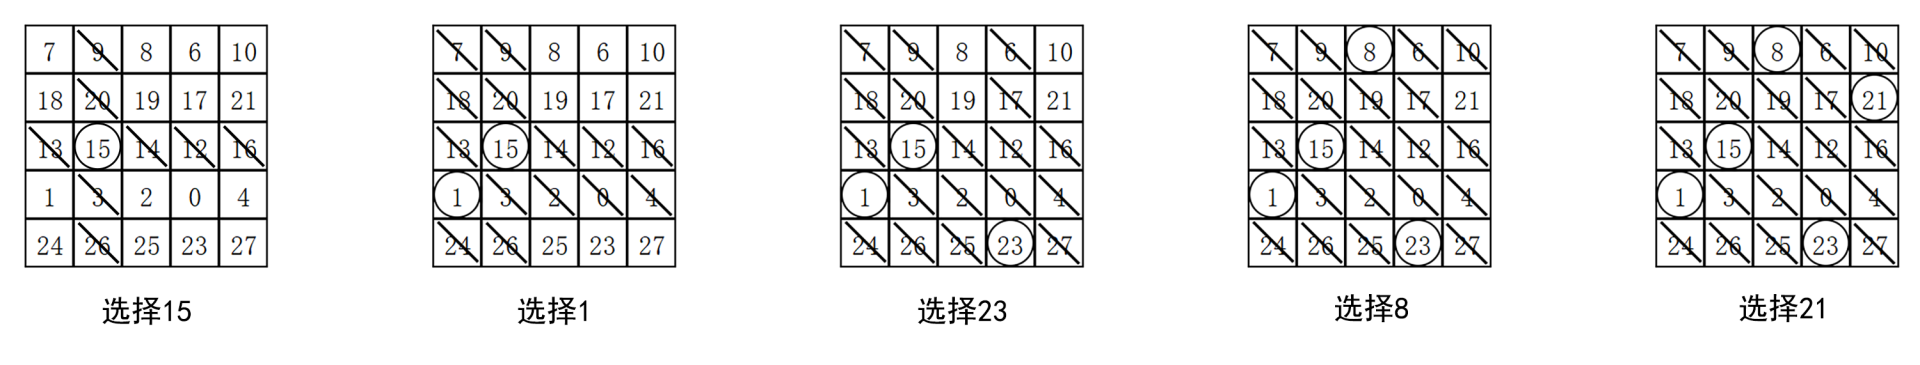
\includegraphics[scale=0.2]{./picture/game_sample.png}
\end{figure}

对打上圈的数求和,即 $15+1+23+8+21 = 68 = n$。

可以证明,任意的选法都能够使和为 $68$。

据此,该矩阵满足此条件。

\sample{2}{输入}

\begin{lstlisting}
1
4 60
\end{lstlisting}

\sample{2}{输出}

\begin{lstlisting}
-1
\end{lstlisting}

\sample{2}{解释}

可以证明不存在这样的矩阵。

\para{数据范围}

对 100\% 的数据,$1\leq T\leq 10$,$1\leq n\leq 500$,$1\leq k\leq 10^9$。

\begin{center}
	\begin{tabu}{c|c|c}
		\tabucline[2pt]{-}
		子任务编号 & 限制 & 分数 \\
		\tabucline[1.2pt]{-}
		Subtask 0 & $T = 1, n = 1, k = 1$ & 10 \\ \hline
		Subtask 1 & $T = 1, 1 \le n \le 5, 1 \le k \le 5$ & 15  \\ \hline
		Subtask 2 & $1 \le T \le 10, 1 \le n \le 100, 1 \le k \le 10^5$ & 25  \\ \hline
		Subtask 3 & $1 \le T \le 10, 1 \le n \le 500, 1 \le k \le 10^9$ & 50\\
		\tabucline[2pt]{-}
	\end{tabu}
\end{center}

\newprob{F}{初生几何}{mathematics}

\para{题目描述}

\begin{figure}[H]
\centering
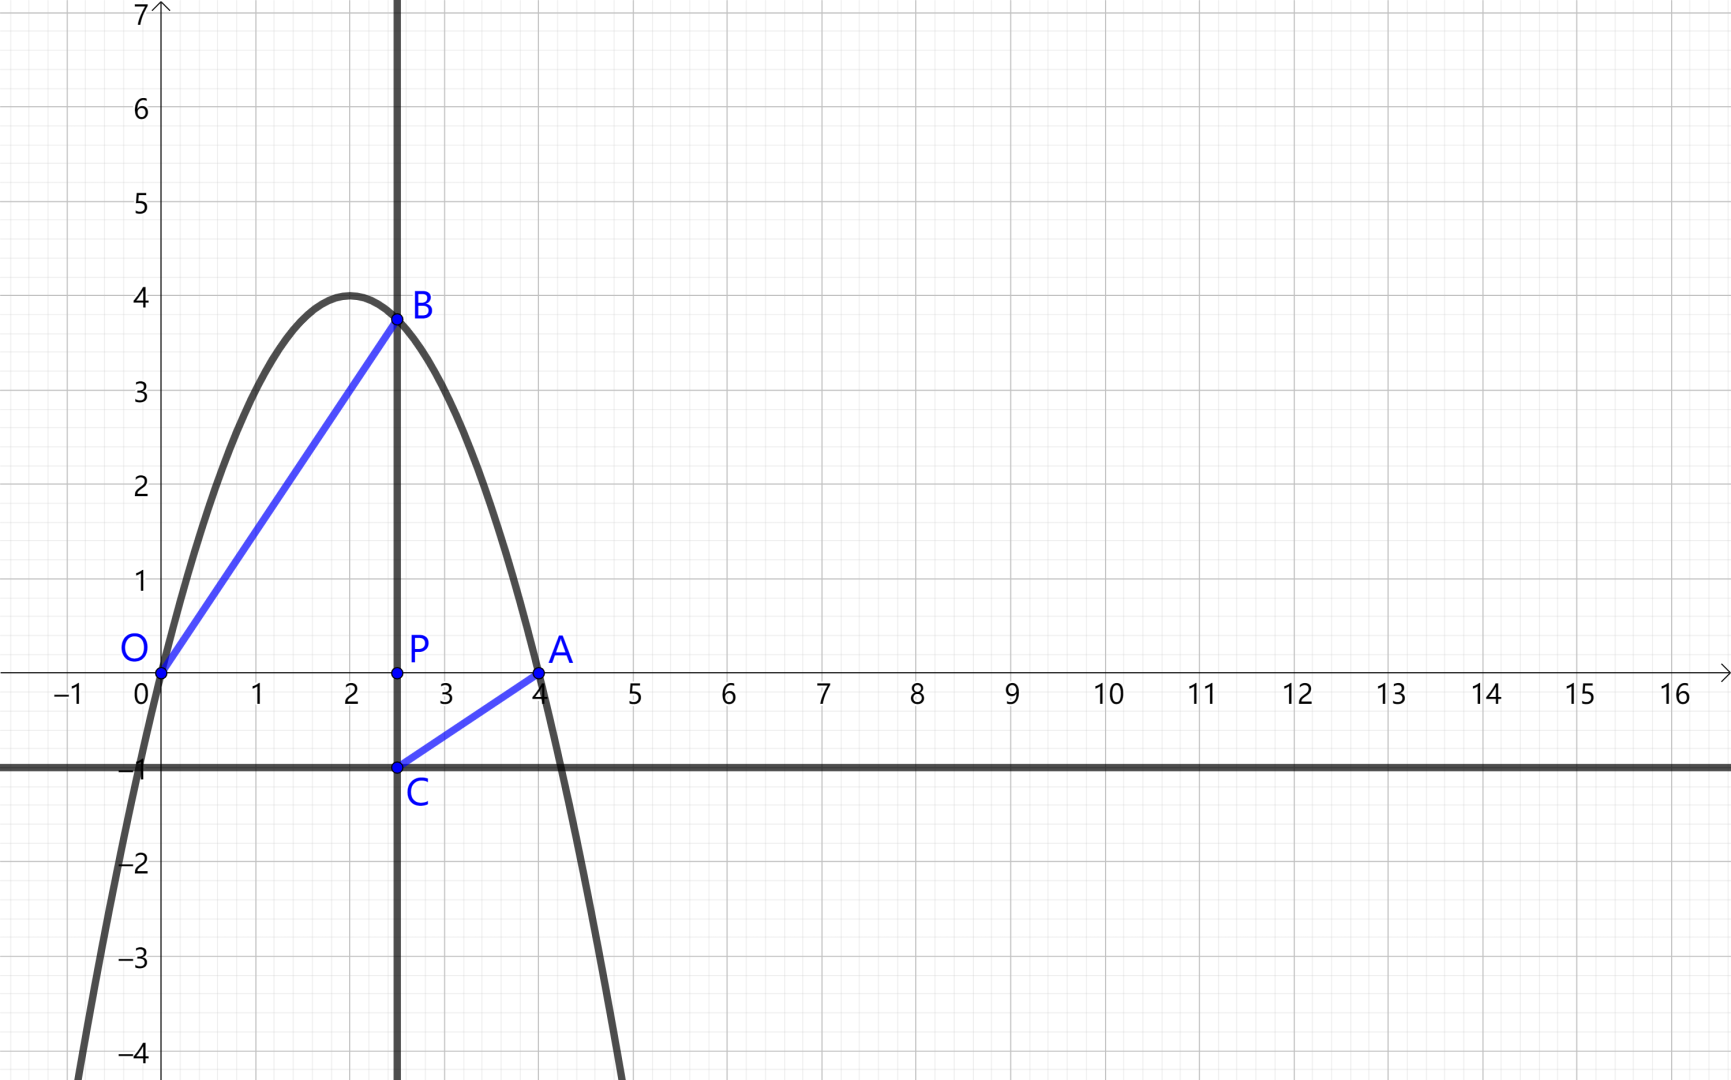
\includegraphics[scale=0.25]{./picture/mathematics.png}
\end{figure}

在平面直角坐标系中,抛物线 $ y = -x^2 + kx $ 与直线 $ y = -1 $ 相交。抛物线过与原点相异的点 $\mathrm{A}$。

设\textbf{线段} $\mathrm{OA}$ 上一点 $\mathrm{P}$,过点 $\mathrm{P}$ 作 $y$ 轴平行线交抛物线于 $\mathrm{B}$,交 $y = -1$ 于 $\mathrm{C}$。

求 $\mathrm{P}$ 的坐标,使得 $\mathrm{OB}^2 + \mathrm{AC}^2$ 最大,并求这个最大值。

\para{输入格式}

每个测试点包含多组测试数据。

每个测试点的第一行包含一个整数 $ T $,代表测试数据组数。

每组测试数据仅包含两个由空格隔开的\textbf{正整数} $ a, b $,表示 $ k = \frac{a}{b} $。

\para{输出格式}

对于每组测试数据,输出 $\mathrm{OB}^2 + \mathrm{AC}^2$ 的最大值。

本题有两种输出方式,你可以采取其中的任意一种:

\begin{itemize}
\item 方式 $ 1 $:

输出一个\textbf{实数},代表 $\mathrm{OB}^2 + \mathrm{AC}^2$ 的最大值。

设你的答案为 $ x $,标准答案为 $ X $,则绝对误差 $ \Delta x = \left| X - x \right| $,相对误差 $ E_r = \frac{\Delta x}{X} $。

当 $ \Delta x \le 10^{-5} $ 或 $ E_r \le 10^{-5} $ 时,你的答案即可被判定为正确答案。

\item 方式 $ 2 $:

输出答案对 $ 998244353 $ 取模的值。

可以证明答案是一个有理数。

\textit{什么是答案对 $ 998244353 $ 取模的值?}

\textit{设答案为 $ \frac{P}{Q}$($P, Q \in \mathbf{N}^*$),可以证明有且仅有一个整数 $ R $($R \in [0, 998244353) $) 使得 $ R \times Q \equiv P \pmod {998244353} $,$ R $ 即为 $ \frac{P}{Q} $ 对 $ 998244353 $ 取模的值。你只需要输出 $ R $。}

\end{itemize}

\sample{1}{输入}

\begin{lstlisting}
1
365 254
\end{lstlisting}

\sample{1}{输出}

\begin{lstlisting}
2.29900771698543729578
\end{lstlisting}

\sample{2}{输入}

\begin{lstlisting}
1
365 254
\end{lstlisting}

\sample{2}{输出}

\begin{lstlisting}
391310912
\end{lstlisting}

\sample{1, 2}{解释}

样例 1 为输出方式 1 的示例,而样例 2 为输出方式 2 的示例。你只需要任意选择一种方式输出。

\para{数据范围}

对于 $ 100\% $ 的数据,有 $ 1 \le T \le 10^5, 0 < a, b \le 10^4 $。

\begin{center}
	\begin{tabu}{c|c|c}
		\tabucline[2pt]{-}
		子任务编号 & 特殊性质 & 分数 \\ \tabucline[1.2pt]{-}
		Subtask 0 & $b = 1$ & 20 \\ \hline
		Subtask 1 & 无 & 80 \\ \tabucline[2pt]{-}
	\end{tabu}
\end{center}

\newprob{G}{排序算法}{sort}

\para{题目背景}

某日,小陈同学翻出了不知多久以前写的老代码,内容如下:

\begin{lstlisting}
#include <iostream>
#include <vector>

int main() {
  int n;
  std::cin >> n;
  std::vector<int> a(n);
  for (int i = 0; i < n; ++i) {
    std::cin >> a[i];
  }

  for (int i = 0; i < n; ++i) {
    for (int j = 0; j < n; ++j) {
      if (a[i] < a[j]) {
        std::swap(a[i], a[j]);
      }
    }
  }

  for (int i = 0; i < n; ++i) {
    std::cout << a[i] << ' ';
  }

  return 0;
}

\end{lstlisting}

小陈同学非常困惑,他想知道他的程序是否正确,并且想知道 \texttt{std::swap(a[i], a[j]);} 执行了多少次。

\para{题目描述}

给定正整数 $ n $ 与一个长度为 $ n $ 的序列 $ a $,如果题目背景中的程序可以将序列 $ a $ 排序为\textbf{严格不下降}序列,则输出 \texttt{YES},并输出程序中 \texttt{std::swap(a[i], a[j]);} 这一条语句的运行次数,否则输出 \texttt{NO}。

\para{输入格式}

第一行包含一个正整数 $ n $,第二行包含 $ n $ 个由空格隔开的正整数 $ a_1, a_2, \dots, a_n $。

\para{输出格式}

如果题目背景中的程序可以将序列 $ a $ 重新排序为\textbf{严格不下降}序列,则在第一行输出 \texttt{YES},并在第二行输出一个整数,代表程序中 \texttt{swap(a[i],a[j]);} 这一条语句的运行次数,否则输出 \texttt{NO}。

\sample{1}{输入}

\begin{lstlisting}
5
5 4 3 2 1
\end{lstlisting}

\sample{1}{输出}

\begin{lstlisting}
YES
10
\end{lstlisting}

\para{数据范围}

对于 $100\%$ 的数据,有 $1 \le n \le 2 \times 10^5$,$1 \le a_i \le 10^9 $。

\begin{center}
	\begin{tabu}{c|c|c|c}
		\tabucline[2pt]{-}
		子任务编号 &  限制 & 特殊性质 & 分数 \\ \tabucline[1.2pt]{-}
		Subtask 0 & $1 \le n \le 10^3$ & 无 & 20 \\ \hline
		Subtask 1 & $1 \le n \le 2 \times {10}^5$ & A & 30 \\ \hline
		Subtask 2 & $1 \le n \le 2 \times 10^5$ & 无 & 50 \\ \tabucline[2pt]{-}
	\end{tabu}
\end{center}

特殊性质 A:对 $1 \le i < j \le n$,$a_i \neq a_j$。

\newprob{H}{购买车券}{sparkarte}

\para{题目背景}

\begin{wrapfigure}{r}{5.4cm}
	\centering
	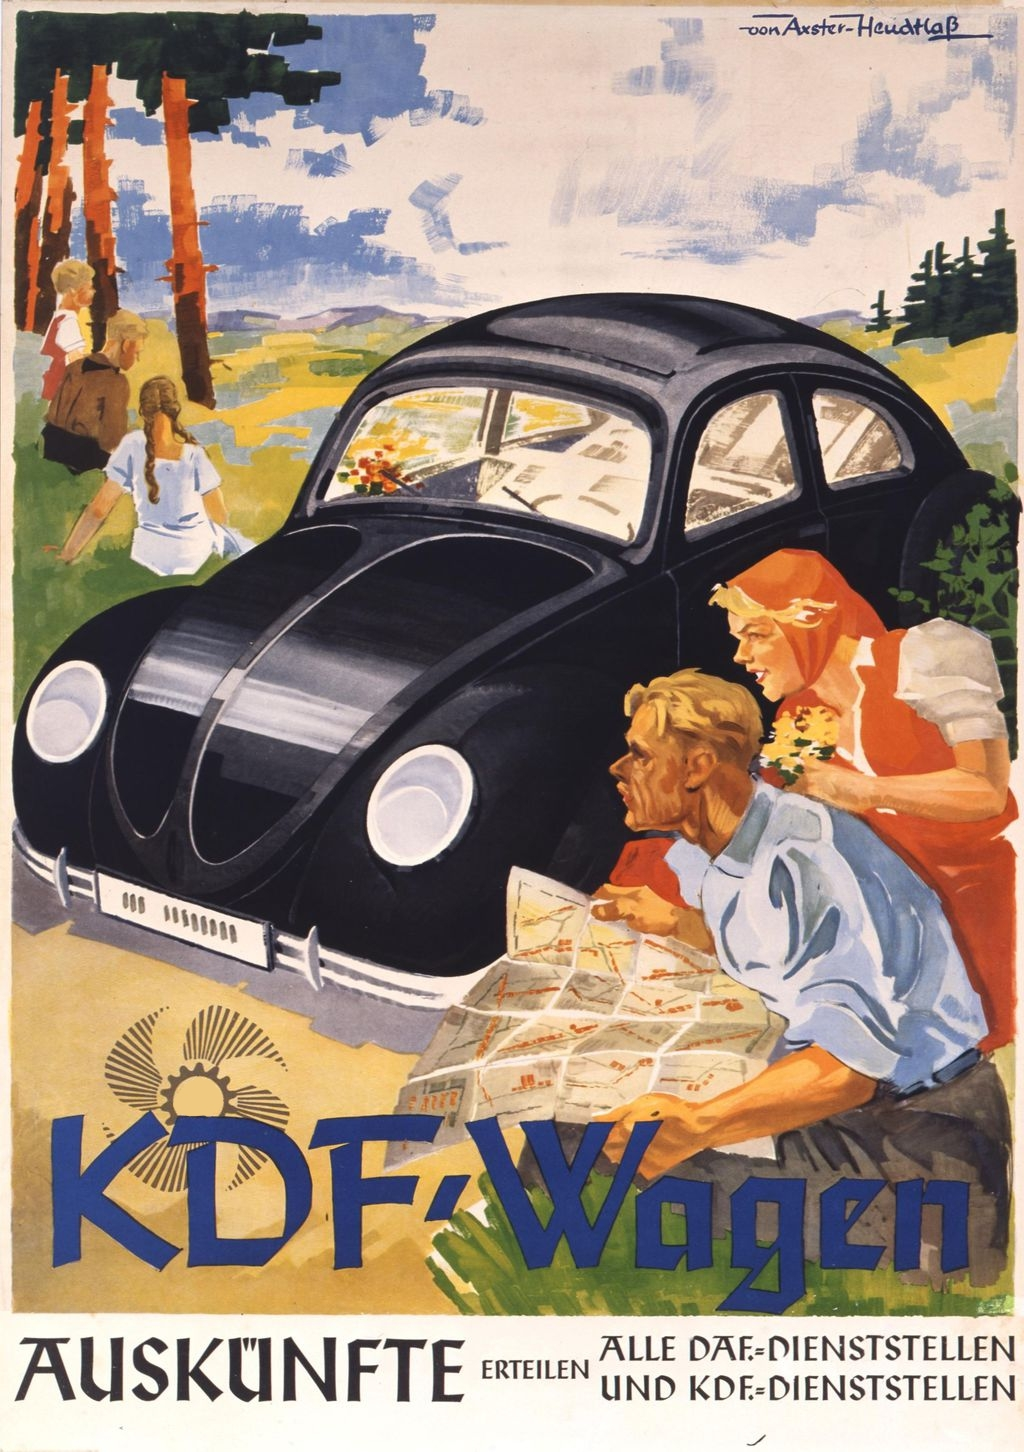
\includegraphics[scale=0.18]{./picture/sparkarte.jpg}
\end{wrapfigure}

“力量来自欢乐”是 1930 年代德国的一个旅游公司,他们在本土推出了一款汽车,由费迪南德·保时捷一手设计,其宗旨是让每一个德国人民都用得上一辆汽车。

为了促进德国人民购买“力量来自欢乐”牌汽车,德国政府推出了一种“购车券”:每一张券的价值是 5 帝国马克,购买的人可以通过类似集邮的方式,当其所拥有的券价值总和和一辆车同价(990帝国马克)时,就能够兑换一辆“力量来自欢乐”牌汽车。

然而,和梅福券一样,随着 1939 年战争的爆发,大部分的“购车券”都成为了空头支票,被政府用作了扩军的资本。

\para{题目描述}

您收集了 $n$ 张“购车券”,并假设某些“购车券”之间有一定的关联关系,一共有 $n - 1$ 对\textbf{双向的}关联关系。

为了让这个问题简单有趣,您保证了这些“购车券”\textbf{不存在}循环的关联关系(即关联关系不成环),并且如果对两张“购车券”增加一对关联关系之后,只含有\textbf{唯一}循环的关联关系。

对于一张“购车券”,当你\textbf{至多}未购买一张和其相关联的“购车券”时,你就可以购买该“购车券”。

当你购买了所有的“购车券”时,你便能够兑换一辆“力量来自欢乐”牌汽车。

您想知道:有多少种购买“购车券”的方案,使得您能够兑换一辆汽车。

有趣的是,由于答案可能很大,您只想知道其对 $998,244,353$ 取模的结果。

\para{输入格式}

从标准输入读入数据。

第一行一个正整数 $n$,含义见题目描述。

接下来 $n-1$ 行,每行两个正整数 $u_i,v_i$,表示第 $u_i$ 张和第 $v_i$ 张“购车券”之间有一对关联关系。

\para{输出格式}

输出到标准输出中。

共一行,包含一个整数,为购买“购车券”的方案数对 $998,244,353$ 取模的值。

\sample{1}{输入}

\begin{lstlisting}
3
1 2
1 3
\end{lstlisting}

\sample{1}{输出}

\begin{lstlisting}
4
\end{lstlisting}

\sample{1}{解释}

\begin{figure}[H]
\centering
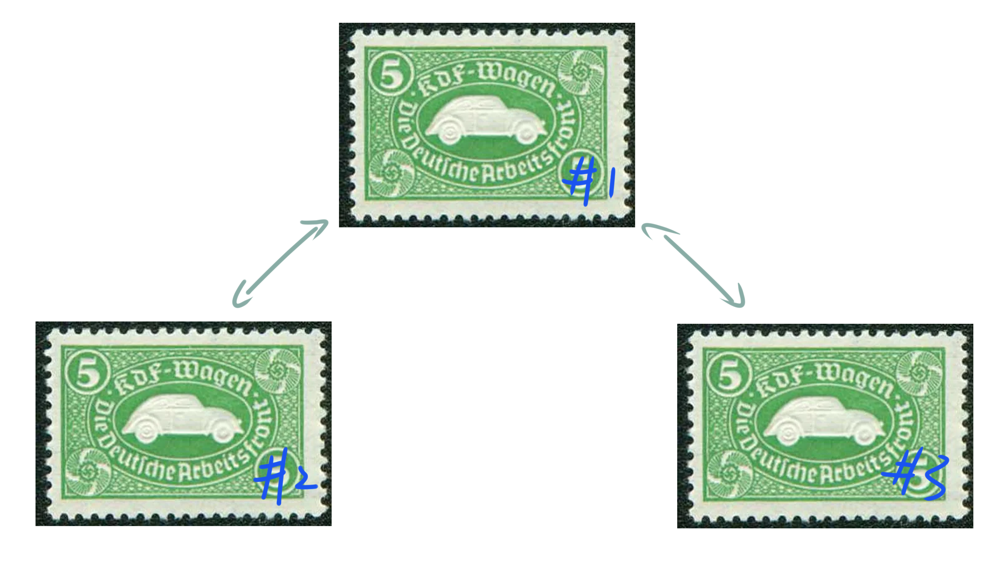
\includegraphics[scale=1.0]{./picture/sparkarte_sample.png}
\end{figure}

您可以先购买 $3$ 号购车券,此时对于 $1$ 号购车券,您只剩一张关联的购车券还未拥有($2$ 号购车券),因此您能够购买 $1$ 号购车券。总共的购买顺序为 $(3,1,2)$。

类似的,您也能以 $(2,1,3),(2,3,1),(3,2,1)$ 的顺序购买,一共 $4$ 种购买方式。

\sample{2}{输入}

\begin{lstlisting}
5
1 2
1 3
2 4
2 5
\end{lstlisting}

\sample{2}{输出}

\begin{lstlisting}
28
\end{lstlisting}

\sample{3}{输入}

\begin{lstlisting}
8
1 2
1 3
3 4
4 5
4 6
6 7
7 8
\end{lstlisting}

\sample{3}{输出}

\begin{lstlisting}
392
\end{lstlisting}

\sample{4}{输入}

\begin{lstlisting}
18
14 3
16 11
6 10
8 7
1 3
4 17
3 17
4 16
9 13
15 10
13 2
18 9
17 12
12 10
7 5
3 18
7 12
\end{lstlisting}

\sample{4}{输出}

\begin{lstlisting}
289685999
\end{lstlisting}

\para{数据范围}

对于 $ 100\% $ 的数据,保证 $1 \le n \le 2 \times 10^5 $,$1 \le u_i, v_i \le n$,$u_i \neq v_i$。

\begin{center}
	\begin{tabu}{c|c|c|c}
		\tabucline[2pt]{-}
		子任务编号 &  限制 & 特殊性质 & 分数 \\ \tabucline[1.2pt]{-}
		Subtask 0 & $1 \le n \le 10$ & 无 & 13 \\ \hline
		Subtask 1 & $1 \le n \le 3 \times 10^3$ & 无 & 22 \\ \hline
		Subtask 2 & $1 \le n \le 2 \times 10^5$ & A & 13  \\ \hline
		Subtask 3 & $1 \le n \le 2 \times 10^5$ & B & 12 \\ \hline
		Subtask 4 & $1 \le n \le 2 \times 10^5$ & 无 & 40 \\ \tabucline[2pt]{-}
	\end{tabu}
\end{center}

特殊性质 A:保证每张“购车券”至多只有两张“购车券”相关联。

特殊性质 B:保证存在至少一张“购车券”与 $n-1$ 张“购车券”相关联。

\para{提示}

\udot{本题 IO 量较大,请酌情选用较为高效的 IO 方式。}

\newprob{I}{花腔星云}{coloratura}

\para{题目背景}

\textit{And up there in the heavens 高高在上 于天堂之中}

\textit{Galileo and those pining for the moon 伽利略和前人们伫立于此}

\textit{Know it's a slow burn 深知过程必然缓慢}

\textit{Through Pioneer and Helix 掠过先驱者号与螺旋星云}

\textit{Oumuamua, Heliopause, and Neptune 奥陌陌,日球层顶与海王星}

\textit{We're a slow-burning tune 韵律缓慢燃烧}

\textit{But we'll get there 故事延绵亘久}

—— Coloratura 花腔星云,Coldplay

\begin{figure}[H]
\centering
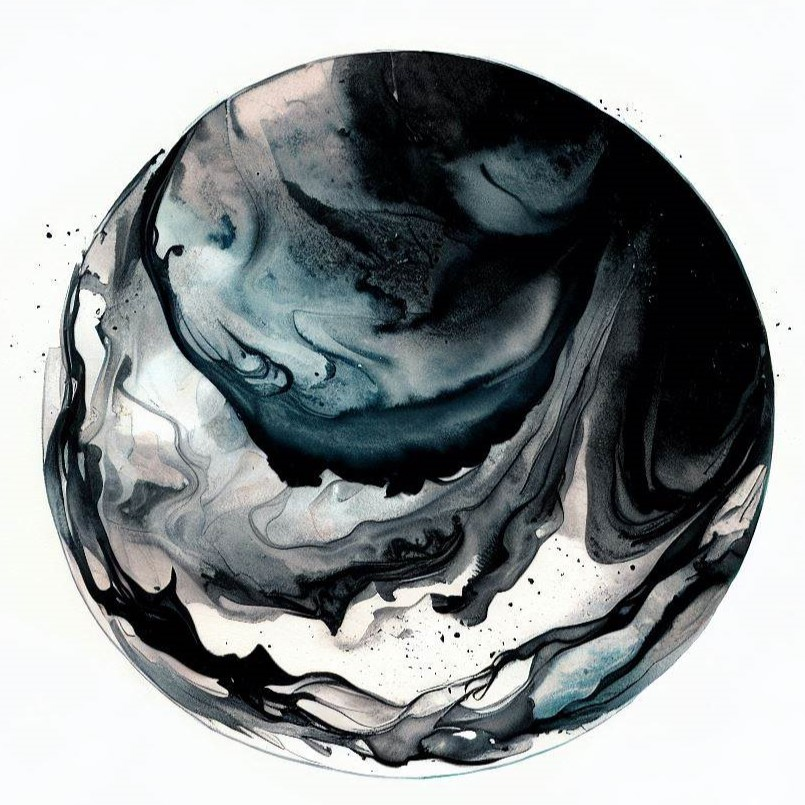
\includegraphics[scale=0.4]{./picture/coloratura.jpg}
\end{figure}

\para{题目描述}

可爱的序列扑满看到了一片美丽的花腔星云。

在这个宇宙一共有 $3$ 种行星,编号为 $1, 2, 3$,而这片星云有 $n$ 颗行星,第 $i$ 颗行星的种类为 $a_i$。

接下来,序列扑满用 $q$ 种方式欣赏这片星云。第 $i$ 种欣赏方式用一个三元组 $\left(l_i, r_i, v_i\right)$ 表示,代表第 $l_i$ 颗至第 $r_i$ 颗行星的种类编号的乘积,除以 $4$ 的余数为 $v_i$。

现在可爱的序列扑满将行星的个数 $n$,欣赏方式数量 $q$ 和每种欣赏方式的三元组 $\left(l_i, r_i, v_i\right)$ 告诉了你,你能不能猜出花腔星云中的每颗行星可能的种类呢?

由于序列扑满很可爱,所以记录一定没有出错,也就是说存在一种行星种类的情况,满足序列扑满的所有欣赏方式。

\para{输入格式}

从标准输入读入数据。

第一行两个整数 $n, q$,含义见题目描述。

接下来 $q$ 行,每行三个整数 $l_i, r_i, v_i$,代表给定的三元组。

\para{输出格式}

输出到标准输出中。

输出 $n$ 个正整数,代表一个满足条件的序列 $a_j$。

\udot{本题使用 Special Judge}。你可以输出\udot{任意}满足条件的序列。

\sample{1}{输入}

\begin{lstlisting}
6 3
1 3 3
2 4 2
5 6 1

\end{lstlisting}

\sample{1}{输出}

\begin{lstlisting}
3 1 1 2 3 3

\end{lstlisting}

\sample{1}{解释}

第一种欣赏方式 $\left(1, 3, 3\right)$ 即 $\left(3 \times 1 \times 1\right) \bmod 4 = 3$。

第二个欣赏方式 $\left(2, 4, 2\right)$ 即 $\left(1 \times 1 \times 2\right) \bmod 4 = 2$。

第三个欣赏方式 $\left(5, 6, 1\right)$ 即 $\left(3 \times 3\right) \bmod 4 = 1$。

据此,所有的欣赏方式都得到了满足,3, 1, 1, 2, 3, 3 是一组合法的情况。

\sample{2}{输入}

\begin{lstlisting}
11 4
3 10 3
1 2 2
2 3 1
7 8 1

\end{lstlisting}

\sample{2}{输出}

\begin{lstlisting}
2 3 3 1 3 1 3 3 3 1 1

\end{lstlisting}

\sample{3}{输入}

\begin{lstlisting}
9 4
1 3 2
3 6 2
5 9 2
3 6 2
\end{lstlisting}

\sample{3}{输出}

\begin{lstlisting}
2 1 3 2 1 3 2 1 3
\end{lstlisting}

\para{数据范围}

对于 $100\%$ 的数据,$1 \le n \le 2 \times {10}^4$,$0 \le q \le 2 \times {10}^4$,$0 \le v_i < 4$。

\begin{center}
	\begin{tabu}{c|c|c}
		\tabucline[2pt]{-}
		子任务编号 &  限制 & 分数 \\ \tabucline[1.2pt]{-}
		Subtask 0 & $q = 0$ & 2 \\ \hline
		Subtask 1 & $1 \le n, q \le 10$ & 13  \\ \hline
		Subtask 2 & $1 \le n, q \le 10^2$,$v_i = 2$ & 17 \\ \hline
		Subtask 3 & $1 \le n, q \le {10}^3$,$v_i \in \{1, 3\}$ & 27 \\ \hline
		Subtask 4 & $1 \le n, q \le 2 \times {10}^4$ & 41 \\ \tabucline[2pt]{-}
	\end{tabu}
\end{center}

\newprob{J}{妄想感伤}{sadness}

\para{题目描述}

\para{输入格式}

\para{输出格式}

\para{数据范围}

\end{document}